\documentclass[a4paper]{scrartcl}

\usepackage[T1]{fontenc}
%\usepackage{wallpaper}
\usepackage{cook}

\newcommand\kochbuchauthor{Sebastian Preisner und Nicole Neumann}
\newcommand\kochbuchurl{http://www.calyrium.org/}
\newcommand\kochbuchtitle{Fitness Küche}
\newcommand\kochbuchversion{Ver. 0.1}

\newcommand{\caps}{www.calyrium.org}

\setcounter{secnumdepth}{-1} % um die nummerierung von sections zu unterbinden und trotzdem die PDF-Bookmarks zu haben

% Schriftarten fuer Ueberschriften
\usepackage{aurical}
\usepackage{calligra}
\usepackage{yfonts}
\usepackage{uncial}
\usepackage{rustic}
%\usepackage{emerald}
%\usepackage{rotunda}
%\usepackage{inslrmin}
%\usepackage{pbsi}
%\usepackage{egothic}
%\usepackage{carolmin}
%%\usepackage{chancery}
%\usepackage{sqrcaps}


\definecolor{darkblue}{rgb}{0,0,.5}
\usepackage[ % muss letztes Package sein!
	pdftitle={\kochbuchtitle},%
	pdfauthor={\kochbuchauthor},%
	pdfsubject={Kochbuch},%
	pdfcreator={PDFLaTeX},
	colorlinks=true, urlcolor=darkblue, linkcolor=darkblue, bookmarksopen=true
 ]{hyperref} % 

%\twosided 	% Zweiseitig?

\usekomafont{section}
\addtokomafont{section}{\newpage\centering\vspace*{2cm}\rmfamily\Huge\color{darkred}}

% ============================= Einheiten ==============================
\newcommand{\g}{\,g }
\newcommand{\kg}{\,kg }
\newcommand{\ml}{\,ml }
\renewcommand{\l}{\,l }
\newcommand{\TL}{\,TL }
\newcommand{\EL}{\,EL }
\newcommand{\cm}{\,cm }
\newcommand{\m}{\,m }
\renewcommand{\min}{\,min }
\newcommand{\pkg}{\,Päckchen}

% ============================= Abkuerzungen ==============================
\newcommand{\bzw}{bzw.\@\xspace}
\newcommand{\bzgl}{bzgl.\@\xspace}
\newcommand{\ca}{ca.\@\xspace}
\newcommand{\dah}{d.\thinspace{}h.\@\xspace}
\newcommand{\Dah}{D.\thinspace{}h.\@\xspace}
\newcommand{\ds}{d.\thinspace{}sind\@\xspace}
\newcommand{\evtl}{evtl.\@\xspace}
\newcommand{\ua}{u.\thinspace{}a.\@\xspace}
\newcommand{\Ua}{U.\thinspace{}a.\@\xspace}
\newcommand{\usw}{usw.\@\xspace}
\newcommand{\va}{vor allem\@\xspace}
\newcommand{\vgl}{vgl.\@\xspace}
\newcommand{\zB}{z.\thinspace{}B.\@\xspace}
\newcommand{\ZB}{Zum Beispiel\xspace}
\newcommand{\sa}{s.\ auch\@\xspace}
\newcommand{\ia}{i.\thinspace{}Allg.\@\xspace}
\newcommand{\su}{s.\ unten\@\xspace}
\newcommand{\uvm}{u.\thinspace{}v.\thinspace{}m.\@\xspace}
\newcommand{\uva}{u.\thinspace{}v.\thinspace{}a.\@\xspace}
\newcommand{\uae}{u.\thinspace{}ä.\@\xspace}
\newcommand{\tk}{TK\@\xspace}

\begin{document}

% entweder die Optionen ausfüllen und mit \maketitle Titelseite erzeugen oder...
%\title{Meine Küche}
%\author{Autor}
%\maketitle

% ... die Titelseite selber zusammenstellen
\pdfbookmark[1]{Titel}{Meine Fitnessküche}
\begin{titlepage}
		\begin{center}
		\textcolor{white}{\\[6.5cm]\bfseries{	\scalebox{5.5}{Fitness} \\[1,5cm]\scalebox{5.5}{Küche} 
				\\[12cm]	\scalebox{1.8}{\kochbuchurl}} \\ \centering\vspace*{1cm}\copyright \ 2015 \kochbuchauthor \ \ \kochbuchversion}
		\end{center}
		\ThisCenterWallPaper{1.52}{./bilder/start2.jpg}
		%\begin{figure}[H]% einfügen der Grafik
			%\centering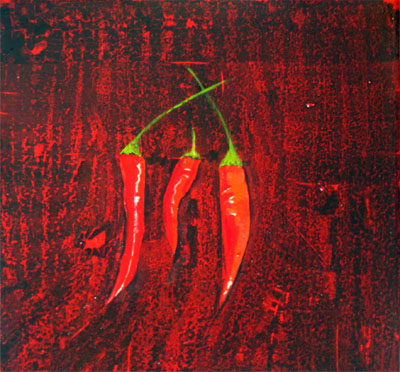
\includegraphics[width=0.95\textwidth]{./bilder/start2.jpg}
			%\centering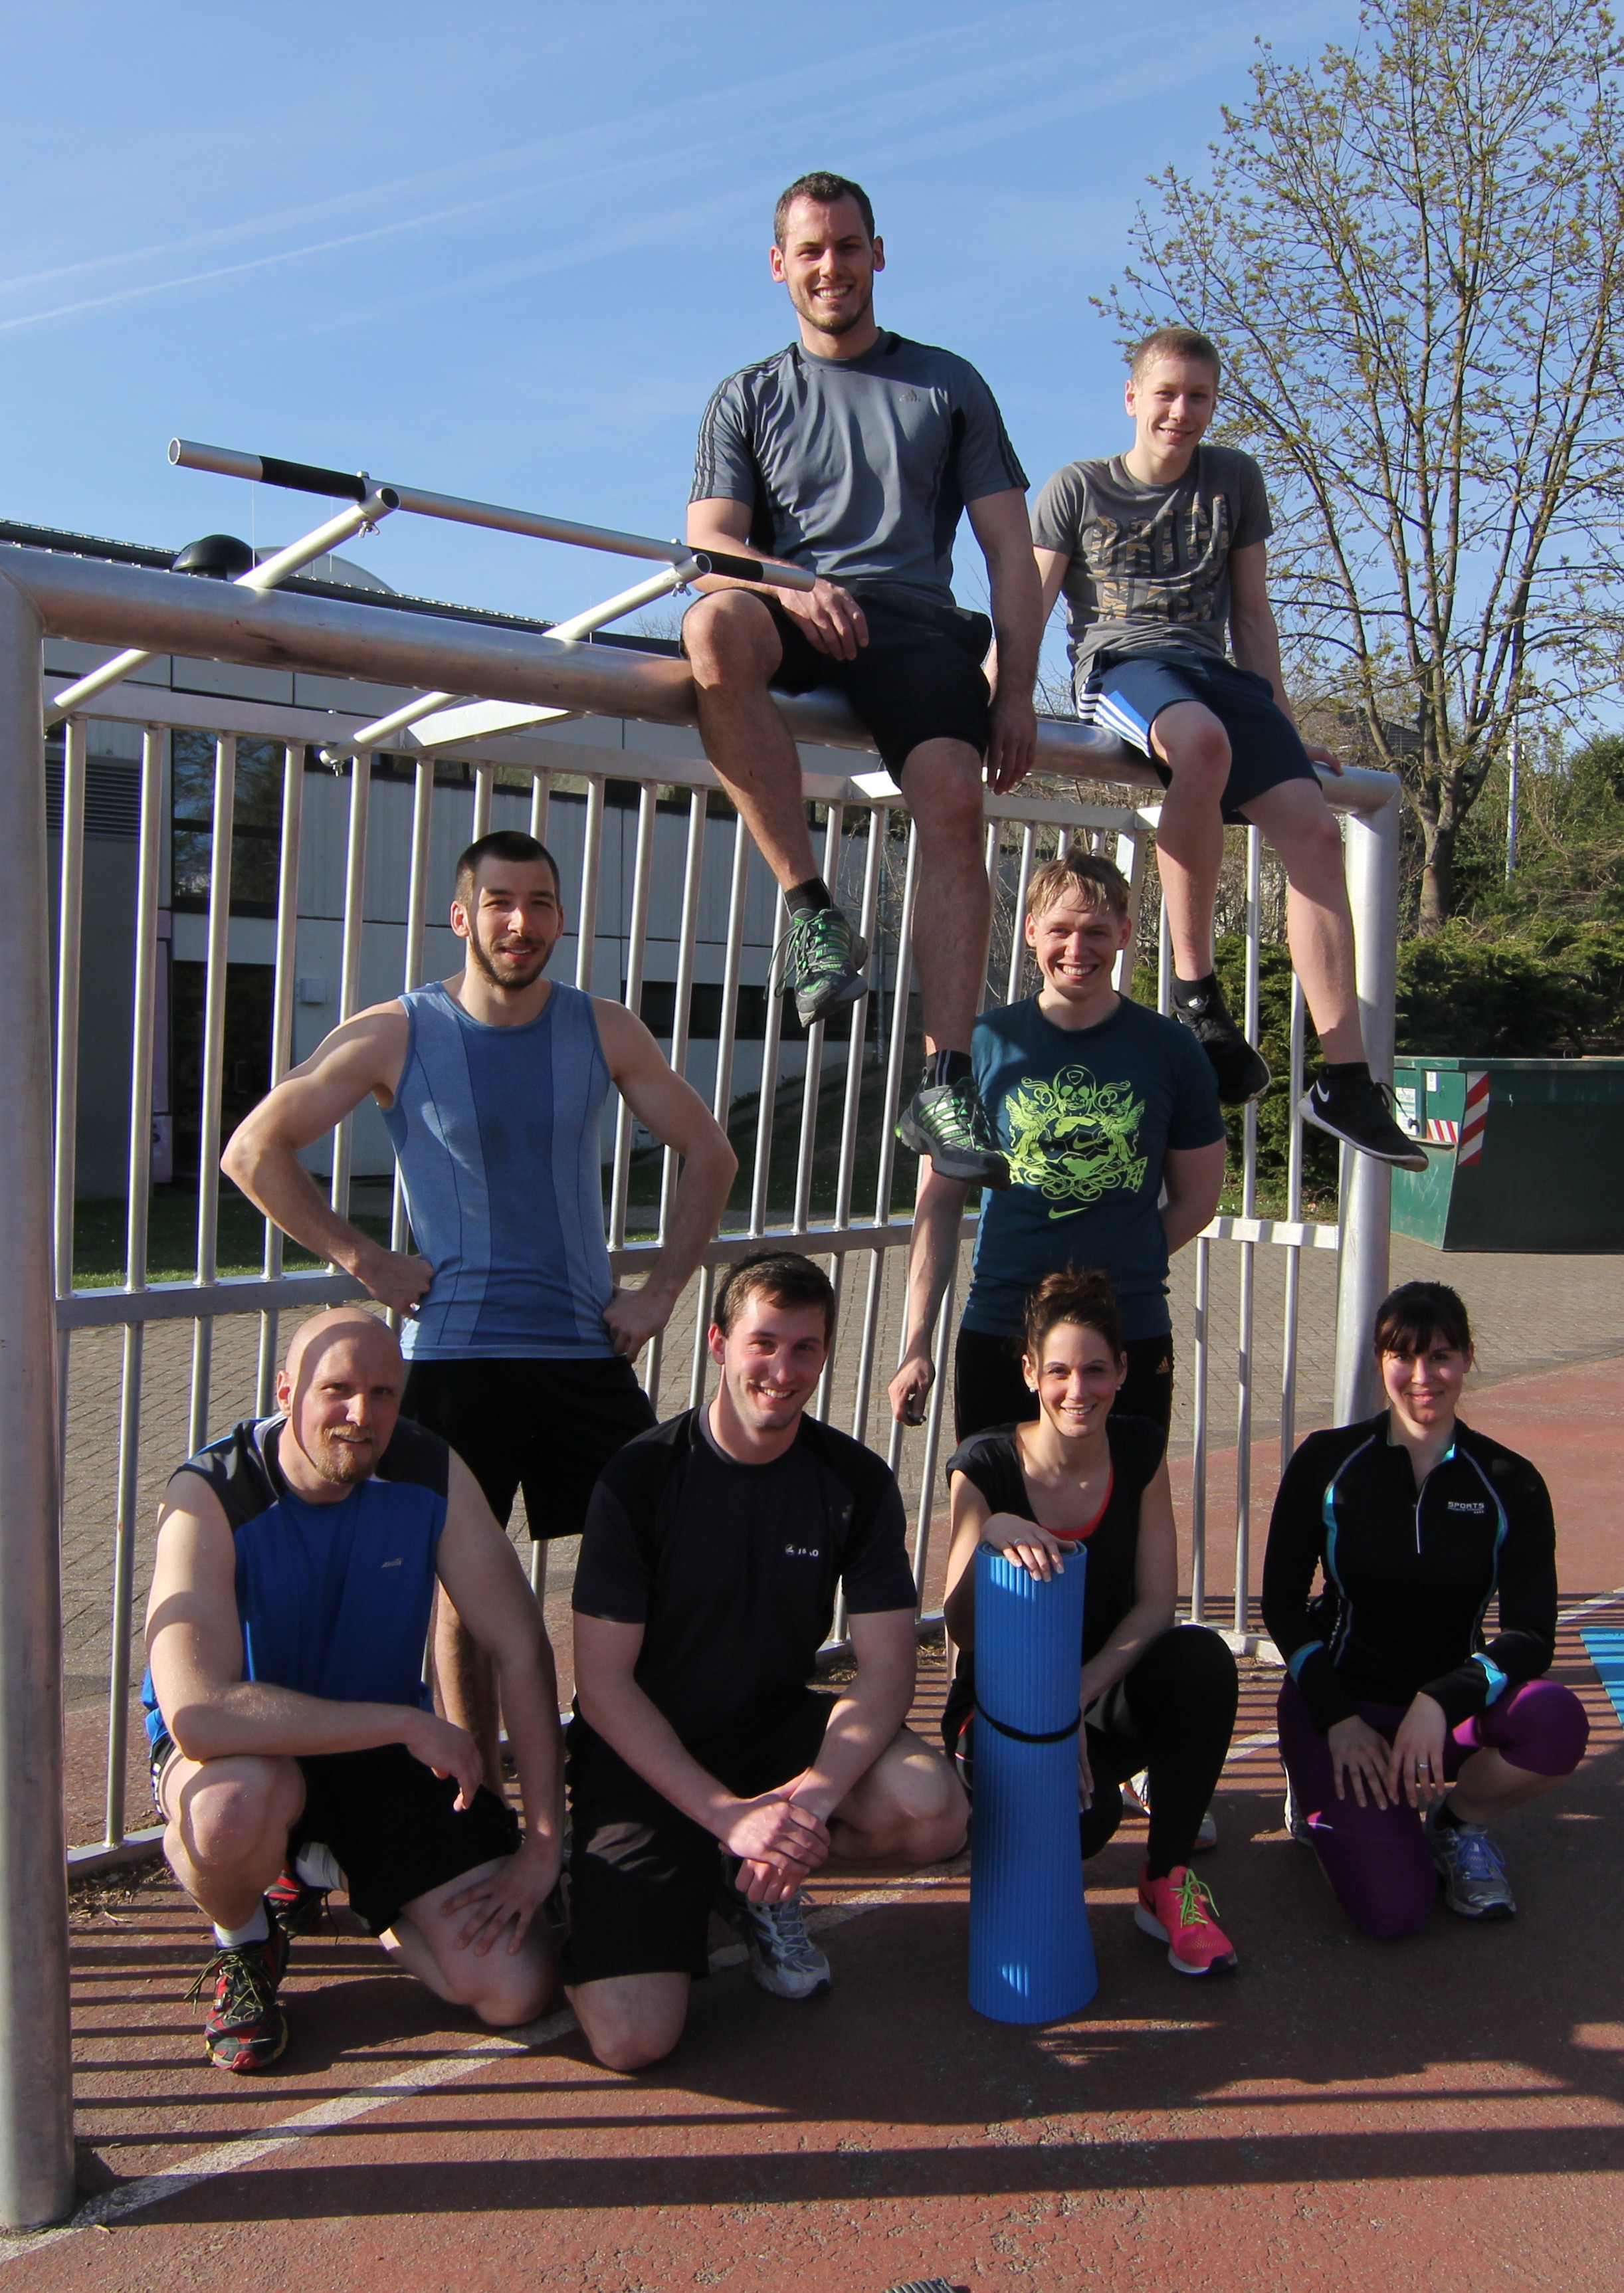
\includegraphics[height=0.94\textheight]{./bilder/start.jpg}
		%\end{figure}
\newpage
%\centering\vspace*{3cm}\copyright \ 2011 \kochbuchauthor
\end{titlepage}

\pdfbookmark[1]{Inhaltsverzeichnis}{toc}
\tableofcontents

% Standardfarbe, -schriftart für die Überschrift
\recipecolor{FFB649}

% Schriftart der Ueberschrift
%\recipefont{\rustfamily}
%\recipefont{\calligra}
%\recipefont{\Fontskrivan}
\recipefont{\Fontlukas}
%\recipefont{\Fontamici}
%\recipefont{\cminfamily}
%\recipefont{\rmfamily}
%\recipefont{\ECFJD}

% wenn \twosided aktiv ist (bei Zweiseitig ist die ungerade Zahl immer auf der Vorderseite)
% müssen hier soviele newpages einfügen bis die erste Sektion auf einer ungeraden Seite beginnt
\newpage~
\subsection*{\centering Danksagung}
\begin{quote}
Vielen Dank an \emph{Stefan Gabauer} der mit seinem Chili Cook Book\footnote{\url{http://sourceforge.net/projects/chilicookbook}} die \LaTeX-Stil-Vorlage von \emph{Christian Gatzlaff} zugänglich gemacht hat und uns somit das Werkzeug zur Erstellung dieses Fitnesskochbuchs in die Hand gegeben hat.\\

Wir möchten uns natürlich bei all den Kreativen Köpfen bedanken die ihre Rezeptideen mit uns geteilt haben und uns so zu dieser Zusammenstellung Inspiriert haben.
\vspace{2cm}

\subsection*{\centering Lizenz}
\begin{center}
"`Fitness Küche"'\\
\textit{Dieses Kochbuch zeigt das gesunde Ernährung auch gut schmecken kann!}\\
Copyright (C) 2015 Sebastian Preisner\\

\begin{center}
	\href{http://creativecommons.org/licenses/by-nc-sa/3.0/de/}{
\includegraphics{cclogo.png}}
\end{center}

Fitness Küche von Sebastian Preisner und Nicole Neumann steht unter einer\\ \href{http://creativecommons.org/licenses/by/4.0/}{Creative Commons Namensnennung 4.0 International Lizenz.}\\
\url{http://creativecommons.org/licenses/by/4.0/}
\end{center}
\end{quote}
%%%%%%%%%%%%%%%%%%%%%%%%%%%%%%%%%%%%%%%%%%%%%%%%%%%%%%%%%%%%%%%%%%%%%%%%%%%%%%%%%%%%%%%%%%%%%%%


\section{Konservieren} %%%%%%%%%%%%%%%%%%%%%%%%%%%%%%%%% Konservieren

\section{Frühstück} %%%%%%%%%%%%%%%%%%%%%%%%%%%%%%%%% Konservieren


\section{Suppen} %%%%%%%%%%%%%%%%%%%%%%%%%%%%%%%% Suppen

\section{Salate} %%%%%%%%%%%%%%%%%%%%%%%%%%%%%%%% Salate
%\input{./rezepte/BrombeerenGarnelenSalat.tex}

\section{Hauptgerichte} %%%%%%%%%%%%%%%%%%%%%%%%%%%%%%%% Hauptgerichte
% ====== Rezeptname und die Quelle ======
\begin{recipe}[]{ Thunfischfrikadellen mit Asia-Salat }{ Freeletics Ernährungsguid }

% ====== Zeit, Personen und Schärfe ======
%\timerecipe{ca. 1}         % Zubereitungszeit in Stunden
\timerecipe[Minuten]{15}    % oder in Minuten
\personcount{1}        		% Personenanzahl
\spicecount{0}              % Schaerfe von 5

% ====== Zutaten ======
\ingredient{150\g Thunfisch in der Dose}
\ingredient{30\g Haferflocken oder Hafermehl}
\ingredient{1 Ei}
\ingredient{1/2 Zwiebel}
\ingredient{1 Pak Choi (\ca 200\g)}
\ingredient{1 Frühlingszwiebel}
\ingredient{100\g Soja- oder Mungobohnensprossen}
\ingredient{2 \EL Sesam (\ca 20\g)}
\ingredient{1 daumengroßes Stück Ingwer}
\ingredient{1/2 Limette}
\ingredient{3 \EL Sojasauce}

         % ====== Zubereitung ======    
\step
Den Thunfisch mit einer Gabel zerpflücken. Haferflocken in einem Mixer auf höchster Stufe zu einer Art Mehl verarbeiten. Zwiebeln abziehen und klein schneiden. Den Sesam währenddessen in einer Pfanne ohne Fett auf mittlerer Hitze \ca 3 Minuten anrösten. 

\step
Thunfisch, Haferflocken, Ei und Zwiebelwürfel gründlich vermengen. Aus der so entstehenden Masse werden nun 4 gleichgroße Frikadellen geformt. 

\step 
Öl in einer Pfanne bei mittlerer Hitze heiß werden lassen und die Thunfischfrikadellen von jeder Seite \ca 4 Minuten braten.\\ 
Währenddessen Pak Choi, Paprika, Frühlingszwiebel und -falls nötig- Sprossen waschen, trocken tupfen.

\tippbox{Frische Sprossen schmecken einfach am besten. Gibt es oft in großen Supermärkten zu erwerben oder beim Asialaden um die Ecke.}

\step
Pak Choi und Paprika in Streifen schneiden, Frühlingszwiebel in Ringe schneiden und mit den Sprossen und dem Sesam mischen. 

\step 
Den Ingwer nach dem schälen auf einer Reibe fein raspeln und zusammen mit dem Saft der ausgepressten Limette und der Sojasauce auf den Salat geben.

\tippboxtip{Dies ist ein umrahmter Tipp um noch ein paar Zusatzinformationen und weitere Anregungen dem Rezept beizufügen.} 
% Tipp in extra Rahmen mit dem Wort "Tipp:" am Anfang

         % ====== Bild ======
% Grafik fuer das Rezept koennen so eingefuegt werden:
% wenn kein Bild vorhanden ist, bitte diese Zeile auskommentiert lassen.
%\graphic{./bilder/todo.jpg}
\end{recipe}
% ====== Rezeptname und die Quelle ======
\begin{recipe}[]{ Putenbruststreifen mit Erdnusschilisauce }{ Freeletics Nutrationguid }

% ====== Zeit, Personen und Schärfe ======
%\timerecipe{ca. 1}         % Zubereitungszeit in Stunden
\timerecipe[Minuten]{35}    % oder in Minuten
\personcount{2}        		% Personenanzahl
\spicecount{1}              % Schaerfe von 5

% ====== Zutaten ======
\ingredient{400\g Puten- oder Hänchenbrustfilet}
\ingredient{300\g Blumenkohl}
\ingredient{100\g Lauch}
\ingredient{4 Möhren}
\ingredient{200\ml Kokosmilch (ungesüßt)}
\ingredient{8\EL Erdnussbutter (ungesüßt)}
\ingredient{2 Knoblauchzehe}
\ingredient{2 daumengroße Stück Ingwer (40\g)}
\ingredient{1 Limette}
\ingredient{1\TL Chilliflocken oder -ringe}
\ingredient{4\TL Raps- oder Olivenöl}
\ingredient{Salz, Pfeffer}

         % ====== Zubereitung ======    
\step
Puten- oder Hänchenbrustfilet mit kalten Wasser abbrausen, trockentupfen und in \ca 1\cm dicke Streifen schneiden. Den Blumenkohl in Scheiben schneiden. Den Lauch waschen, trockentupfen und in Scheiben schneiden. Möhren schälen und in Scheiben schneiden.
 
\step
In einer Pfanne auf mittlerer Hitze 2\TL Olivenöl erhitzen und darin die Filetstreifen und das Gemüse \ca 2 Minuten von jeder Seite anbraten. Das Fleisch herausnehmen und beiseite legen. 150\ml Wasser auf das Gemüse geben und köcheln lassen bis das Wasser verdampft ist (\ca 5 \min)
\tippbox{Das Fleisch auf einem im Backofen vorgeheizten Teller bei 50 Grad in den Backofen.}

\step
Für die Sauce den Knoblauch und Ingwer schälen und in dünne Scheiben schneiden. Die Zitrone/Limette halbieren und auspressen. In einem Topf bei mittlerer Hitze 1\TL Olivenöl heiß werden lassen und den Knoblauch, Ingwer und die Cihili \ca 3 \min anbraten.

\step
Die Sauce mit Kokosmilch ablöschen, kurz aufkochen lassen und dann vom Herd nehmen. Nun wird die Erdnusscreme und der Limettensaft eingerührt, danach mit Salz und Pfeffer abschmecken.

\step
Putenstreifen mit Gemüse und Erdnusssauce anrichten und  genießen.

% Tipp in extra Rahmen mit dem Wort "Tipp:" am Anfang
\tippboxtip{Dies ist ein umrahmter Tipp um noch ein paar Zusatzinformationen und weitere Anregungen dem Rezept beizufügen.} 

         % ====== Bild ======
% Grafik fuer das Rezept koennen so eingefuegt werden:
% wenn kein Bild vorhanden ist, bitte diese Zeile auskommentiert lassen.
\graphic{./bilder/Putenstreifen_mit_Erdnusschilisauce.jpg}
\end{recipe}
%\input{./rezepte/GebrateneChili-NudelnmitEiundPilzen.tex}

\section{Saucen} %%%%%%%%%%%%%%%%%%%%%%%%%%%%%%%%%%%%%%% Soucen
%\input{./rezepte/Sambal.tex}
%\input{./rezepte/Chilichutney.tex}
%\input{./rezepte/ChileconQueso.tex}
%\input{./rezepte/Habanero-Ingwer-Nektarinen-Erdbeer-Sauce.tex}
%\input{./rezepte/Limetten-Minz-Hot-Sauce.tex}
%\input{./rezepte/LemonDrop-AnanasHotSauce.tex}
%\input{./rezepte/Suess-scharfeThaisauce.tex}
%\input{./rezepte/Chili-Apfel-Paste.tex}

\section{Snaks} %%%%%%%%%%%%%%%%%%%%%%%%%%%%%%%% Snaks
%\input{./rezepte/SchnelleHabisandwiches.tex}

\section{Süßes} %%%%%%%%%%%%%%%%%%%%%%%%%%%%%%%% Süßes
% ====== Rezeptname und die Quelle ======
\begin{recipe}[]{ Brownie Delux }{ \href{https://www.youtube.com/channel/UCR_dfR8wJBmsVkQFDa3PDcQ}{Moin Yamina auf Youtube} }

% ====== Zeit, Personen und Schärfe ======
%\timerecipe{ca. 1}         % Zubereitungszeit in Stunden
\timerecipe[Minuten]{10}    % oder in Minuten
%\personcount{4}        		% Personenanzahl
%\spicecount{3}              % Schaerfe von 5

% ====== Zutaten ======
\ingredient{200\g gemahlene Mandeln}
\ingredient{200\g Kakao}
\ingredient{250\g getrocknete Datteln}
\ingredient{1 Schuss Rum}
\ingredient{Wasser nach bedarf}

         % ====== Zubereitung ======    
\step
Die Datteln mit einem Mixer oder Zauberstab und dem Schuss Rum zerkleinern. Je nach bedarf Wasser hinzufügen bis die Datteln zu einer einheitlichen cremigen Masse werden.

\step
Die gemahlenen Mandeln und den Kakao vermischen und die Dattelmasse hinzufügen. Alles gut vermengen.

\tippbox{Mit einem Löffel habe ich die beste Erfahrung gemacht. Mit den Händen geht es auch und man hat sehr viel zu naschen ;-).}

\step
Die fertige Masse auf einem Backpapier oder Brotpapier verteilen und zu einem flachen Kasten formen. Fertig.

\tippboxtip{Das Rezept kann mit belieben abgewandelt werden. \zB kann man die Masse zu Kugeln formen und mit Haselnüssen füllen. Lass deiner Phantasie freien lauf.} 
% Tipp in extra Rahmen mit dem Wort "Tipp:" am Anfang

         % ====== Bild ======
% Grafik fuer das Rezept koennen so eingefuegt werden:
% wenn kein Bild vorhanden ist, bitte diese Zeile auskommentiert lassen.
%\graphic{./bilder/todo.jpg}
\end{recipe}

\section{Getränke} %%%%%%%%%%%%%%%%%%%%%%%%%%%%%%%%%%%%%%%% Getränke


\section{Smoothies} %%%%%%%%%%%%%%%%%%%%%%%%%%%%%%%%%%%%%%%% Smoothies
% ====== Rezeptname und die Quelle ======
\begin{recipe}[]{ Afterworkout-Beerenmix }{}{}

Dieser Shake zeichnet sich durch den hohen Eiweißgehalt aus und dient so als potentielle Eiweißquelle für nach dem Training, aber auch zur Erfrischung an Warmen Tagen kann der Trink gemacht werden.
% ====== Zeit, Personen und Schärfe ======
%\timerecipe{ca. 1}         % Zubereitungszeit in Stunden
\timerecipe[Minuten]{5}    % oder in Minuten
\personcount{1}        		% Personenanzahl
\spicecount{0}              % Schaerfe von 5

% ====== Zutaten ======
\ingredient{150\g \tk Beerenmix}
\ingredient{500\g Magerquark}
\ingredient{150\ml Wasser}
\ingredient{1 Vanilleschote}


         % ====== Zubereitung ======    
\step
Die Beeren zusammen mit dem Magerquark und dem Wasser in einem Mixer bei höchster Stufe \ca 1\min mixen.

\step
Die Vanilleschote mit einem Messer vorsichtig einschneiden und öffnen. Mit dem Messerrücken die Schote auskratzen und den Inhalt in den Mixer geben. Alles kurz durchmischen und fertig ist der Shake.

\tippboxtip{Dieses Rezept ist als Grundlage zu verstehen. Durch das verändern der Zutaten entstehen immer neue Geschmacksrichtungen. Probiere es aus. } 
% Tipp in extra Rahmen mit dem Wort "Tipp:" am Anfang

         % ====== Bild ======
% Grafik fuer das Rezept koennen so eingefuegt werden:
% wenn kein Bild vorhanden ist, bitte diese Zeile auskommentiert lassen.
%\graphic{./bilder/todo.jpg}
\end{recipe}

\section{Infos und Wissenswertes} %%%%%%%%%%%%%%%%%%%%%%%%%%%%%%%%%%%%%%%%% Info
%\input{./Info.tex}
	
%\end{itemize}

%%%%%%%%%%%%%%%%%%%%%%%%%%%%%%%%%%%%%%%%%%%%%%%%%%%%%%%%%%%%%%%%%%%%%%%%%%%%%%%%%%%%%%%%%%%%%%%
\end{document}